\documentclass[oneside]{book}
\usepackage{xcolor}
\usepackage{graphicx}
\usepackage{subcaption}
\usepackage[inline,shortlabels]{enumitem}
\usepackage{multicol}
\usepackage{multirow}
\usepackage{booktabs,array,adjustbox}

\graphicspath{{./picture/}}

\newcommand{\exercisename}{Latihan}
\newcommand{\solutionname}{Solusi}

\definecolor{main}{RGB}{0,120,2}

%% Exercise with counter
\newcounter{exer}[chapter]
\setcounter{exer}{0}
\renewcommand{\theexer}{\thechapter.\arabic{exer}}
\newenvironment{exercise}[1][]{
  \refstepcounter{exer}
  \par\noindent\textbf{\color{main}{\exercisename} \theexer #1 }\rmfamily}{
  \par\ignorespacesafterend}

\newenvironment{solution}{\par\noindent\textbf{\color{main}\solutionname} \em}{\par}

\begin{document}

\chapter{Digital Transmission}

% Johanes Wilian Ang 1-4
\begin{exercise}
  Contoh soal 1
\end{exercise}

\begin{solution}
  Contoh solusi
\end{solution}

\vspace{12pt}

\begin{exercise}
  Contoh soal
\end{exercise}

\begin{solution}
  Contoh solusi
\end{solution}

\vspace{12pt}

\begin{exercise}
  Contoh soal
\end{exercise}

\begin{solution}
  Contoh solusi
\end{solution}

\vspace{12pt}


\begin{exercise}
  Contoh soal
\end{exercise}

\begin{solution}
  Contoh solusi
\end{solution}

\vspace{12pt}

% Erwin Erikson 5-8
\begin{exercise}

  Gambarlah grafik skema Manchester menggunakan masing-masing aliran data berikut, dengan asumsi bahwa level sinyal terakhir adalah positif. Dari grafik, tebak bandwidth untuk skema ini menggunakan jumlah rata-rata perubahan level sinyal.
  \begin{enumerate}[a)]
    \item 00000000
    \item 11111111
    \item 01010101
    \item 00110011
  \end{enumerate}

  Bandingkan tebakan Anda dengan entri yang sesuai pada Tabel 1.1.

  \begin{table}[htbp]
    \begin{center}
      \centerline{Tabel 1.1: Ringkasan skema pengkodean baris}
      \begin{tabular}{|l|l|c|p{6cm}|}
        \cline{1-4}
        \multirow{2}{*}{Kategori}&\multirow{2}{*}{Skema}&\multicolumn{1}{c|}{Bandwidth}&\multirow{2}{*}{\centerline{Karakteristik}} \\
        & &\multicolumn{1}{c|}{(rata-rata)}& \\
        \cline{1-4}
        Unipolar&NRZ&B=N/2&Mahal, tidak ada sinkronisasi otomatis jika panjang Os atau Is, DC \\
        \cline{1-4}
        \multirow{3}{*}{Unipolar}&NRZ-L&B=N/2&Tidak ada sinkronisasi sendiri jika Os panjang atau 1s, DC \\
        \cline{2-4}
        &NRZ-I&B=N/2&Tidak ada sinkronisasi otomatis selama S, DC \\
        \cline{2-4}
        &Biphase&B=N&Sinkronisasi diri, tidak ada DC, bandwidth tinggi \\
        \cline{1-4}
        Bipolar&AMI&B=N/2&Tidak ada sinkronisasi otomatis untuk OS lama, DC \\
        \cline{1-4}
        \multirow{3}{*}{Multilevel}&2BIQ&B=N/4&Tidak ada sinkronisasi sendiri untuk bit ganda yang sama panjang \\
        \cline{2-4}
        &8B6T&B=3N/4&Sinkronisasi diri, tidak ada DC \\
        \cline{2-4}
        &4D-PAM5&B=N/8&Sinkronisasi diri, tidak ada DC \\
        \cline{1-4}
        Multiline&MLT-3&B=N/3&Tidak ada sinkronisasi otomatis untuk Os yang lama \\
        \cline{1-4}
      \end{tabular}
    \end{center}\vspace*{6px}
  \end{table}\vspace*{8px}

\end{exercise}

\begin{solution}

  Gambar grafik skema Manchester dapat dilihat pada Gambar 1.1.

\begin{figure}[ht]
  \centering
  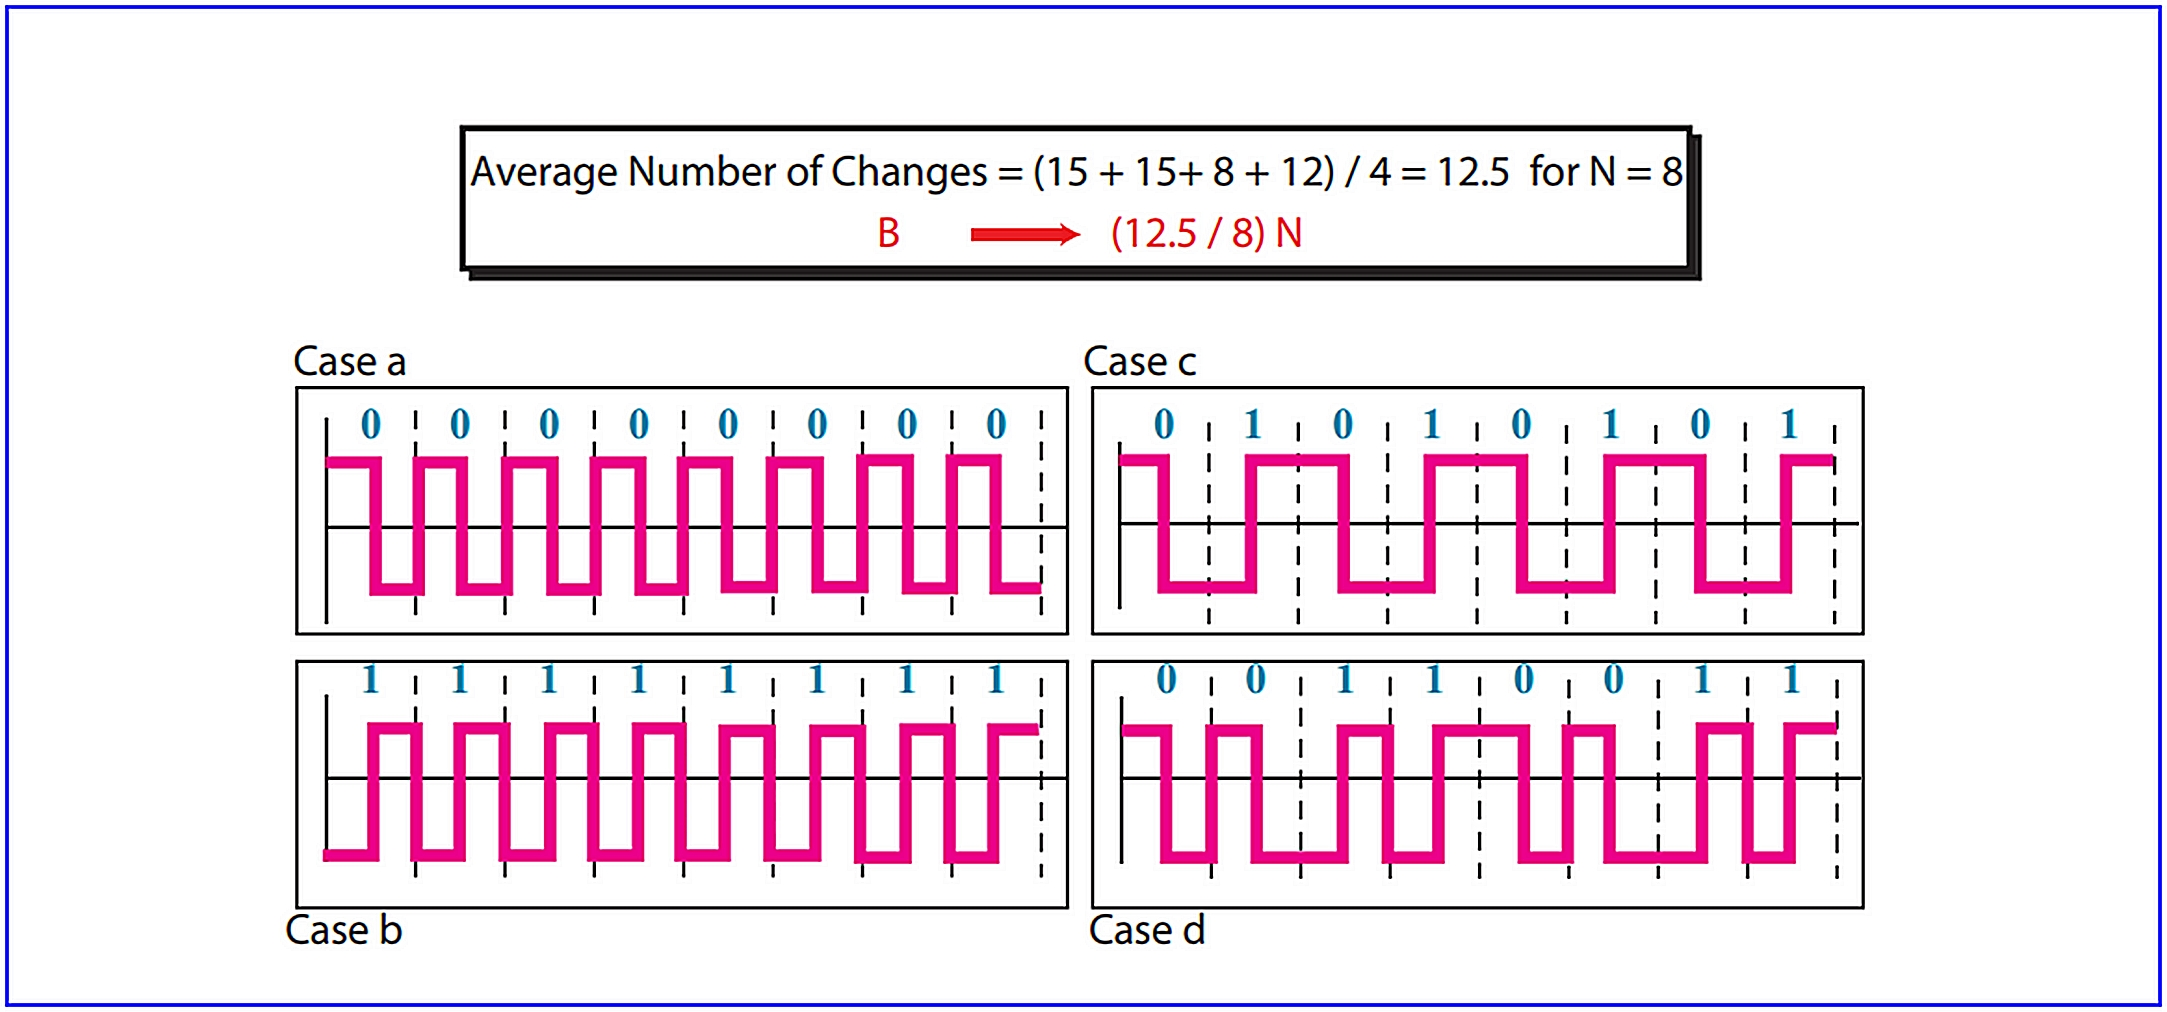
\includegraphics[width=0.9\textwidth]{gbr_solusi_1_5.jpg}
  \centerline{Gambar 1.1: Gambar grafik skema Manchester}\vspace*{2px}
\end{figure}

Bandwidth sebanding dengan (12,5 / 8) N yang berada dalam kisaran pada Tabel 1.1

(B = N hingga B = 2N) untuk skema Manchester.

\end{solution}

\vspace{12pt}

\begin{exercise}

  Gambarlah grafik skema diferensial Manchester menggunakan masing-masing aliran data berikut, dengan asumsi bahwa level sinyal terakhir adalah positif. Dari grafik, tebak bandwidth untuk skema ini menggunakan jumlah rata-rata perubahan level sinyal.
  \begin{enumerate}[a)]
    \item 00000000
    \item 11111111
    \item 01010101
    \item 00110011
  \end{enumerate}

  Bandingkan tebakan Anda dengan entri yang sesuai pada Tabel 1.1.\vspace*{8px}

\end{exercise}

\begin{solution}

  Gambar grafik skema diferensial Manchester dapat dilihat pada Gambar 1.2.

\begin{figure}[ht]
  \centering
  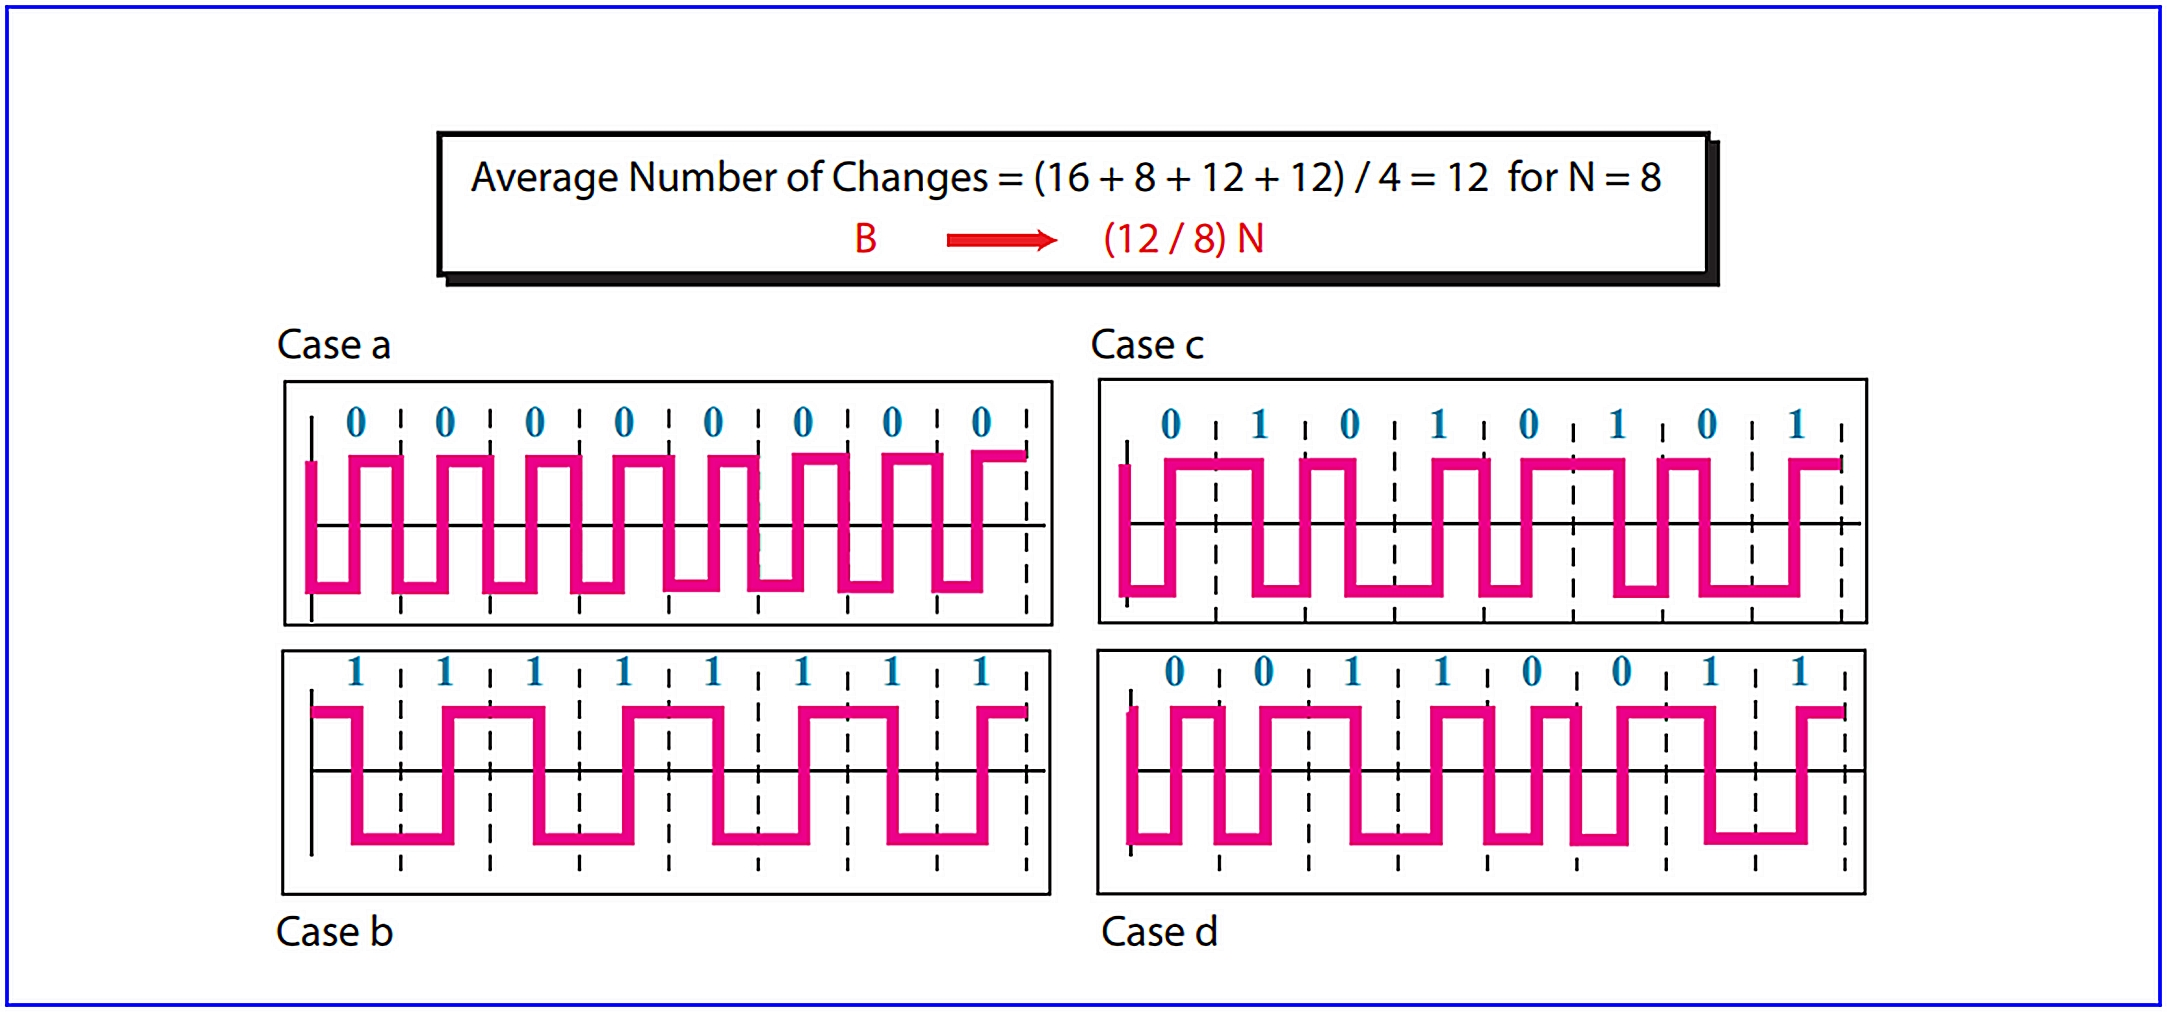
\includegraphics[width=0.9\textwidth]{gbr_solusi_1_6.jpg}
  \centerline{Gambar 1.2: Gambar grafik skema diferensial Manchester}\vspace*{2px}
\end{figure}

Bandwidth sebanding dengan (12/8) N yang berada dalam kisaran pada Tabel 1.1

(B = N ke 2N) untuk skema diferensial Manchester.

\end{solution}

\vspace{12pt}

\begin{exercise}

  Gambarlah grafik skema 2B1Q menggunakan masing-masing aliran data berikut, dengan asumsi bahwa level sinyal terakhir adalah positif. Dari grafik, tebak bandwidth untuk skema ini menggunakan jumlah rata-rata perubahan level sinyal.
  \begin{enumerate}[a)]
    \item 0000000000000000
    \item 1111111111111111
    \item 0101010101010101
    \item 0011001100110011
  \end{enumerate}

  Bandingkan tebakan Anda dengan entri yang sesuai pada Tabel 1.1.\vspace*{8px}

\end{exercise}

\begin{solution}

  Gambar grafik skema 2B1Q dapat dilihat pada Gambar 1.3.

\begin{figure}[ht]
  \centering
  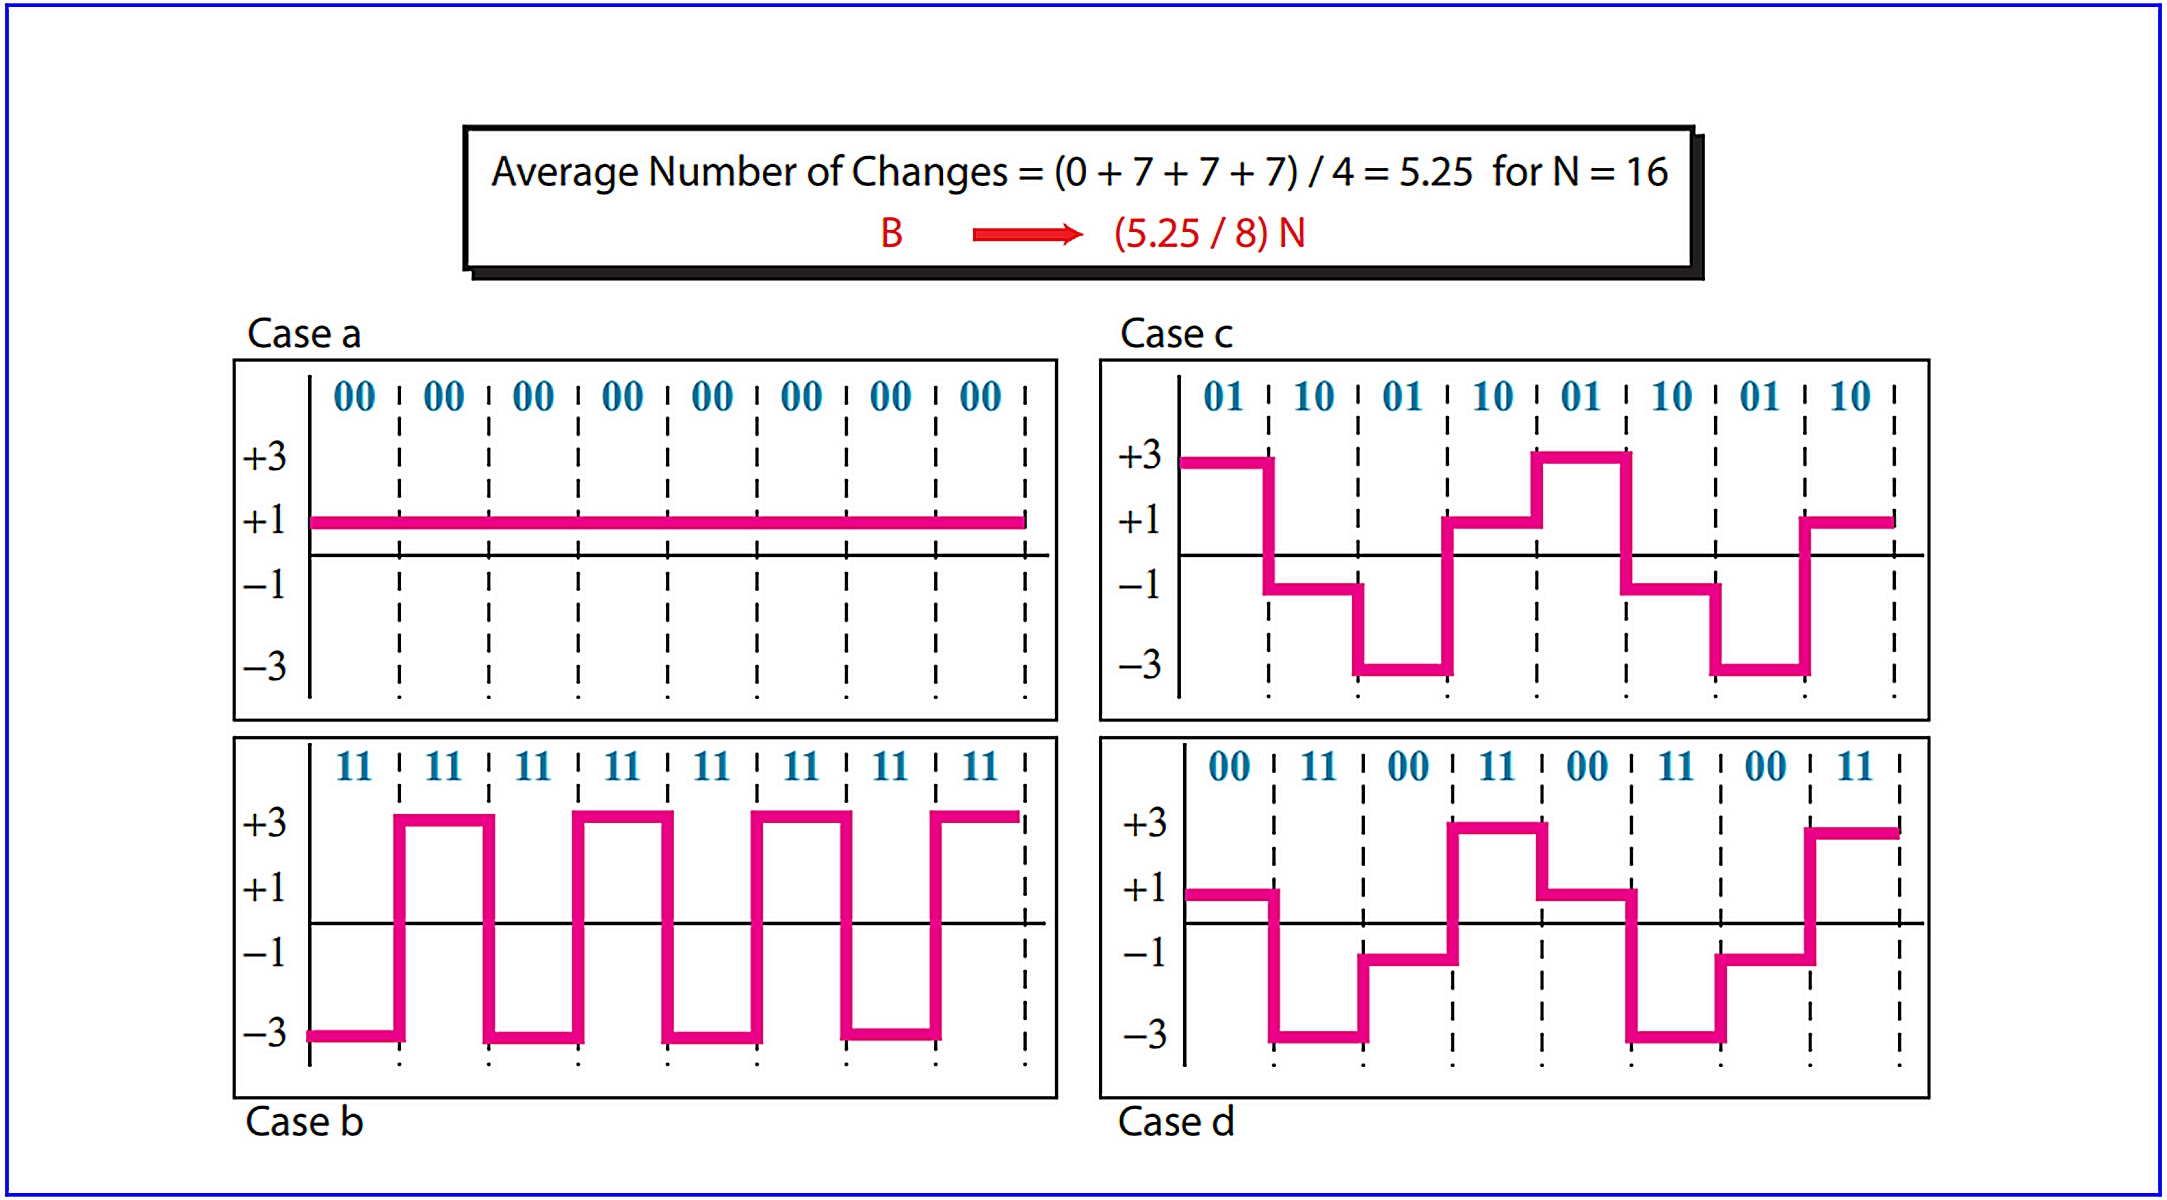
\includegraphics[width=0.9\textwidth]{gbr_solusi_1_7.jpg}
  \centerline{Gambar 1.3: Gambar grafik skema 2B1Q}\vspace*{2px}
\end{figure}

Bandwidth sebanding dengan (5.25 / 16) N yang berada di dalam range pada Tabel 1.1

(B = 0 hingga N/2) untuk 2B/1Q.

\end{solution}

\vspace{12pt}

\begin{exercise}

  Gambarlah grafik skema MLT-3 menggunakan masing-masing aliran data berikut, dengan asumsi bahwa level sinyal terakhir adalah positif. Dari grafik, tebak bandwidth untuk skema ini menggunakan jumlah rata-rata perubahan level sinyal.
  \begin{enumerate}[a)]
    \item 00000000
    \item 11111111
    \item 01010101
    \item 00011000
  \end{enumerate}

  Bandingkan tebakan Anda dengan entri yang sesuai pada Tabel 1.1.\vspace*{8px}

\end{exercise}

\begin{solution}

  Gambar grafik skema MLT-3 dapat dilihat pada Gambar 1.4.

\begin{figure}[ht]
  \centering
  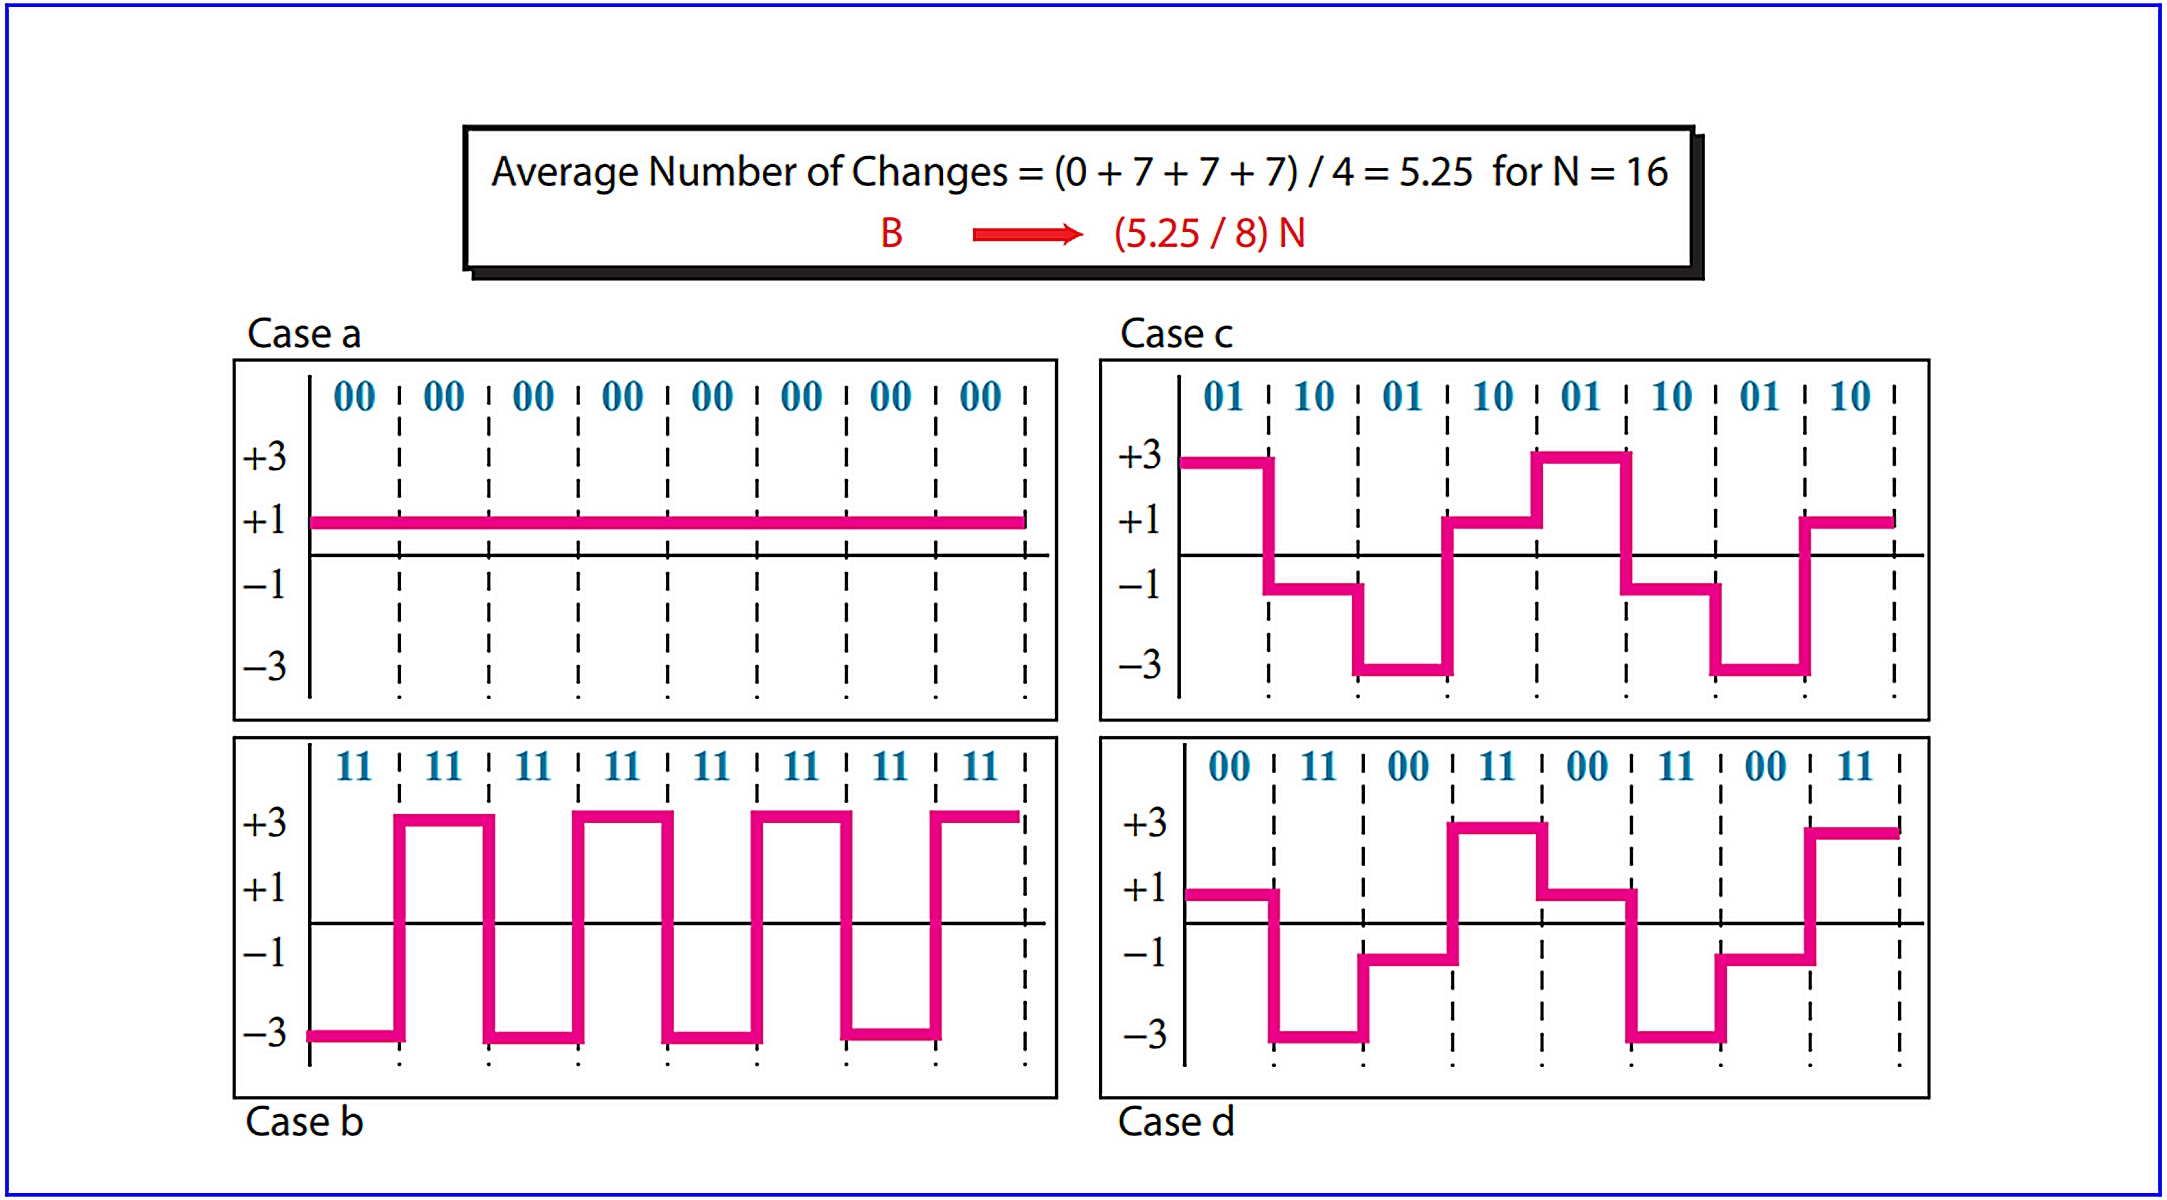
\includegraphics[width=0.9\textwidth]{gbr_solusi_1_7.jpg}
  \centerline{Gambar 1.4: Gambar grafik skema MLT-3}\vspace*{2px}
\end{figure}

Bandwidth sebanding dengan (5.25/8) × N yang berada di dalam kisaran pada Tabel 1.1

(B = 0 hingga N/2) untuk MLT-3.

\end{solution}

\vspace{12pt}

% Johnny 9-12
\begin{exercise}
  Contoh soal 9
\end{exercise}

\begin{solution}
  Contoh solusi
\end{solution}

\vspace{12pt}

\begin{exercise}
  Contoh soal
\end{exercise}

\begin{solution}
  Contoh solusi
\end{solution}

\vspace{12pt}

\begin{exercise}
  Contoh soal
\end{exercise}

\begin{solution}
  Contoh solusi
\end{solution}

\vspace{12pt}

\begin{exercise}
  Contoh soal
\end{exercise}

\begin{solution}
  Contoh solusi
\end{solution}

\vspace{12pt}

% Riani Artika 13-16
\begin{exercise}
  Contoh soal 13
\end{exercise}

\begin{solution}
  Contoh solusi
\end{solution}

\vspace{12pt}

\begin{exercise}
  Contoh soal
\end{exercise}

\begin{solution}
  Contoh solusi
\end{solution}

\vspace{12pt}

\begin{exercise}
  Contoh soal
\end{exercise}

\begin{solution}
  Contoh solusi
\end{solution}

\vspace{12pt}

\begin{exercise}
  Contoh soal
\end{exercise}

\begin{solution}
  Contoh solusi
\end{solution}

\vspace{12pt}

% Muhammad Al Imron 17-20
\begin{exercise}
  Contoh soal 17
\end{exercise}

\begin{solution}
  Contoh solusi
\end{solution}

\vspace{12pt}

\begin{exercise}
  Contoh soal
\end{exercise}

\begin{solution}
  Contoh solusi
\end{solution}

\vspace{12pt}

\begin{exercise}
  Contoh soal
\end{exercise}

\begin{solution}
  Contoh solusi
\end{solution}

\vspace{12pt}

\begin{exercise}
  Contoh soal
\end{exercise}

\begin{solution}
  Contoh solusi
\end{solution}

\chapter{Analog Transmission}

% Rian Sanjaya Nadeak 1-4
\begin{exercise}
  Calculate the baud rate for the given bit rate and type of modulation.
  \begin{itemize}
    \item[a.] 2000 bps, FSK
    \item[b.] 4000 bps, ASK
  \end{itemize}
\end{exercise}

\begin{solution}
  We use the formula $S = (1/r) \times N$, but first we need to calculate the value of r for each case.
  \begin{itemize}
    \item[a.] $r = log_22 = 1 \quad \rightarrow \quad S = (1/1) \times (2000 \textnormal{ bps}) = 2000 \textnormal{ baud}$
    \item[b.] 
  \end{itemize}
\end{solution}

\vspace{12pt}

\begin{exercise}
  Contoh soal
\end{exercise}

\begin{solution}
  Contoh solusi
\end{solution}

\vspace{12pt}

\begin{exercise}
  Contoh soal
\end{exercise}

\begin{solution}
  Contoh solusi
\end{solution}

\vspace{12pt}

\begin{exercise}
  Contoh soal
\end{exercise}

\begin{solution}
  Contoh solusi
\end{solution}

\vspace{12pt}

% R.M. Fikri Ihsan Kurniawan 5-8
\begin{exercise}
  Gambarlah diagram konstelasi untuk kasus-kasus berikut. Temukan amplitudo puncak nilai untuk setiap kasus dan tentukan jenis modulasi (ASK, FSK, PSK, atau QAM).Angka-angka dalam tanda kurung menentukan nilai I dan Q masing-masing.
  \begin{itemize}
    \item[a.] Dua titik di (2, 0) dan (3, 0).
    \item[b.] Dua titik di (3, 0) dan (-3, 0).
    \item[c.] Empat poin di (2, 2), (-2, 2), (-2, -2), dan (2, -2).
    \item[d.] Dua titik di (0 , 2) dan (0, -2).
  \end{itemize}
    
\end{exercise}

\begin{solution}
  \begin{figure}[ht]
  \centering
  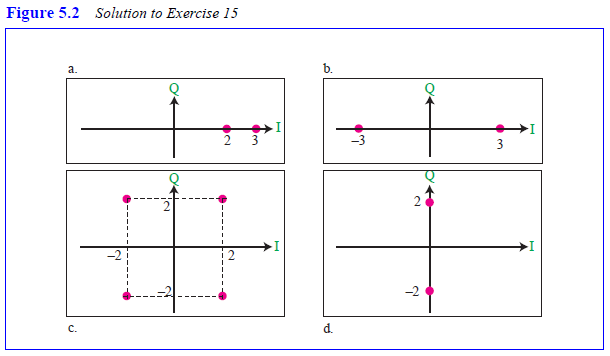
\includegraphics[width=0.9\textwidth]{picture/figure-5.2.png}
  \centerline{Solution of Latihan 2.5}\vspace*{2px}
\end{figure}
\begin{itemize}
    \item[a.] Ada dua amplitudo puncak keduanya dengan fase yang sama (0 derajat). Nilai amplitudo puncak adalah $A_1$ = 2 (jarak antara titik pertama dan titik asal) dan $A_2$ = 3 (jarak antara titik kedua dan titik asal). 
    \item[b.] Hanya ada satu amplitudo puncak (3). Jarak antara masing-masing titik dan asalnya adalah 3. Namun, kami memiliki dua fase, 0 dan 180 derajat.
    \item[c.] Ini dapat berupa QPSK (satu amplitudo, empat fase) atau 4-QAM (satu amplitudo dan empat fase). Amplitudo adalah jarak antara titik dan asal, yaitu $ (2^2 + 2^2)^\frac{1}{2} $ = 2,83.
    \item[d.] Ini juga BPSK. Amplitudo puncaknya adalah 2, tetapi kali ini fasenya adalah 90 dan 270 derajat.
  \end{itemize} 
\end{solution}

\vspace{12pt}

\begin{exercise}
  Berapa banyak bit per baud yang dapat kita kirim dalam setiap kasus berikut jika sinyal: rasi bintang memiliki salah satu dari jumlah titik berikut?
  \begin{itemize}
    \item[a.] 2
    \item[b.] 4
    \item[c.] 16
    \item[d.] 1024
  \end{itemize}
\end{exercise}

\begin{solution}
  Jumlah titik menentukan jumlah level, L. Jumlah bit per baud
adalah nilai r. Oleh karena itu, kami menggunakan rumus r = log$_2$L untuk setiap kasus.
\begin{itemize}
    \item[a.] $ log_2 $2 = 1
    \item[b.] $ log_2 $4 = 2
    \item[c.] $ log_2 $16 = 4
    \item[d.] $ log_2 $1024 = 10
 \end{itemize}
\end{solution}

\vspace{12pt}

\begin{exercise}
 Berapa bandwidth yang dibutuhkan untuk kasus berikut jika kita perlu mengirim 4000 bps? Misalkan d = 1.
  \begin{itemize}
    \item[a.] ASK
    \item[b.] QPSK
    \item[c.] 16-QAM
    \item[d.] 64-QAM
  \end{itemize}
\end{exercise}

\begin{solution}
  Kami menggunakan rumus B = (1 + d) × (1/r) × N, tetapi pertama-tama kita perlu menghitung nilai r untuk setiap kasus.
  \begin{itemize}
    \item[a.] r = 1 → B = (1 + 1) × (1/1) × (4000 bps) = 8000 Hz
    \item[b.] r = 1 → B = (1 + 1) × (1/1) × (4000 bps) + 4 KHz = 8000 Hz
    \item[c.] r = 2 → B = (1 + 1) × (1/2) × (4000 bps) = 2000 Hz
    \item[d.] r = 4 → B = (1 + 1) × (1/4) × (4000 bps) = 1000 Hz
 \end{itemize}
\end{solution}

\vspace{12pt}

\begin{exercise}
  Saluran telepon memiliki bandwidth 4 KHz. Berapa jumlah bit maksimum yang kami? dapat mengirim menggunakan masing-masing teknik berikut? Misalkan d = O
   \begin{itemize}
    \item[a.] ASK
    \item[b.] QPSK 
    \item[c.] 16-QAM
    \item[d.] 64-QAM
    \end{itemize}
\end{exercise}

\begin{solution}
  Kami menggunakan rumus N = [1/(1 + d)] × r × B, tetapi pertama-tama kita perlu menghitung nilai r untuk setiap kasus.
  \begin{itemize}
    \item[a.] r = log$_2$2 = 1 → N= [1/(1 + 0)] × 1 × (4 KHz) = 4 kbps
    \item[b.] r = log$_2$4=2 → N = [1/(1 + 0)] × 2 × (4 KHz) = 8 kbps
    \item[c.] r = log$_2$16= 4 → N = [1/(1 + 0)] × 4 × (4 KHz) = 16 kbps
    \item[d.] r = log$_2$64= 6 → N = [1/(1 + 0)] × 6 × (4 KHz) = 24 kbps
    \end{itemize}
\end{solution}

\vspace{12pt}

% Farhan Ghulam Hadi Saputra 9-12
\begin{exercise}
  Contoh soal 9
\end{exercise}

\begin{solution}
  Contoh solusi
\end{solution}

\vspace{12pt}

\begin{exercise}
  Contoh soal
\end{exercise}

\begin{solution}
  Contoh solusi
\end{solution}

\vspace{12pt}

\begin{exercise}
  Contoh soal
\end{exercise}

\begin{solution}
  Contoh solusi
\end{solution}

\vspace{12pt}

\begin{exercise}
  Contoh soal
\end{exercise}

\begin{solution}
  Contoh solusi
\end{solution}

\chapter{Bandwidth Utilization: Multiplexing and Spreading}

% Hani Khairiyah 1-4
\begin{exercise}
  Asumsikan bahwa saluran suara menempati bandwidth 4 kHz. Kita perlu multipleks 10 saluran suara dengan band penjaga 500 Hz menggunakan FDM. Hitung yang dibutuhkan bandwith?
\end{exercise}

\begin{solution}
  Untuk multipleks 10 saluran suara, kita membutuhkan sembilan band penjaga. Bandwidth yang dibutuhkan kemudian B = (4 KHz) * 10 + (500 Hz) * 9 = 44,5 KHz
\end{solution}

\vspace{12pt}

\begin{exercise}
  Kita perlu mengirimkan 100 saluran suara digital menggunakan saluran pass-band dari 20 KHz. Berapa rasio bit/Hz jika kita tidak menggunakan guard band?
\end{exercise}

\begin{solution}
  Bandwidth yang dialokasikan untuk setiap saluran suara adalah 20 KHz / 100 = 200 Hz. Seperti yang kita lihat di bab sebelumnya, setiap saluran suara digital memiliki kecepatan data 64 Kbps (8000 sampel * 8 bit/sampel). Ini berarti bahwa teknik modulasi kami menggunakan 64.000/200 = 320 bit/Hz.
\end{solution}

\vspace{12pt}

\begin{exercise}
  Dalam hierarki analog Gambar 6.9, temukan overhead bandwidth ekstra untuk guard
band atau kontrol di setiap level hierarki grup, supergrup, grup master, dan
kelompok jumbo.
\end{exercise}

\begin{solution}
  a. Tingkat grup: overhead = 48 KHz (12 * 4 KHz) = 0 Hz
  b. Tingkat supergrup: overhead = 240 KHz (5 * 48 KHz) = 0 Hz
  c. Grup master: overhead = 2520 KHz (10 * 240 KHz) = 120 KHz
  d. Grup Jumbo: overhead = 16,984 MHz (6 * 2,52 MHz) = 1,864 MHz.
\end{solution}

\vspace{12pt}

\begin{exercise}
  Kita perlu menggunakan TDM sinkron dan menggabungkan 20 sumber digital, masing-masing 100 Kbps. Setiap slot keluaran membawa 1 bit dari setiap sumber digital, tetapi satu bit tambahan ditambahkan ke setiap frame untuk sinkronisasi. Jawab pertanyaan berikut
  a. Berapa ukuran bingkai keluaran dalam bit?
  b. Berapa kecepatan bingkai keluaran?
  c. Berapa durasi frame output?
  d. Berapa kecepatan data keluaran?
  e. Berapa efisiensi sistem (rasio bit yang berguna dengan total bit).
\end{exercise}

\begin{solution}
  a. Setiap bingkai keluaran membawa 1 bit dari setiap sumber ditambah satu bit tambahan untuk sinkronisasi. Ukuran bingkai = 20 * 1 + 1 = 21 bit.
  b. Setiap frame membawa 1 bit dari setiap sumber. Kecepatan bingkai = 100.000 bingkai/dtk.\
  c. Durasi bingkai = 1 /(kecepatan bingkai) = 1/100.000 = 10 s
  d. Kecepatan data = (100.000 bingkai/dtk) * (21 bit/bingkai) = 2,1 Mbps
  e. Dalam setiap frame 20 bit dari 21 berguna. Efisiensi = 20/21= 95%
\end{solution}

\vspace{12pt}

% Kevin Antony Kasamilale 5-8
\begin{exercise}
  Contoh soal 5
\end{exercise}

\begin{solution}
  Contoh solusi
\end{solution}

\vspace{12pt}

\begin{exercise}
  Contoh soal 6
\end{exercise}

\begin{solution}
  Contoh solusi
\end{solution}

\vspace{12pt}

\begin{exercise}
  Contoh soal
\end{exercise}

\begin{solution}
  Contoh solusi
\end{solution}

\vspace{12pt}

\begin{exercise}
  Contoh soal
\end{exercise}

\begin{solution}
  Contoh solusi
\end{solution}

\vspace{12pt}

% Annisa Wijaya 9-11
\begin{exercise}
  Contoh soal 9
\end{exercise}

\begin{solution}
  Contoh solusi
\end{solution}

\vspace{12pt}

\begin{exercise}
  Contoh soal
\end{exercise}

\begin{solution}
  Contoh solusi
\end{solution}

\vspace{12pt}

\begin{exercise}
  Contoh soal
\end{exercise}

\begin{solution}
  Contoh solusi
\end{solution}

\vspace{12pt}

% Andrian Syah 12-14 test push ke github
\begin{exercise}
  Contoh soal 12 : Gambar dibawah ini menunjukkan multiplexer dalam sistem TDM sinkron. Setiap slot keluaran adalah
  panjangnya hanya 10 bit (3 bit diambil dari setiap input ditambah 1 bit framing). Apa keluarannya?
  jalur kecil? Bit tiba di multiplexer seperti yang ditunjukkan oleh panah.
\end{exercise}

\begin{figure}[h]
  \centering
  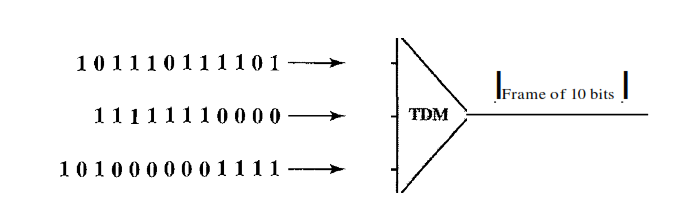
\includegraphics[width=0.9\textwidth]{soal12.png}
\end{figure}

\begin{solution}

\end{solution}

\begin{figure}[h]
  \centering
  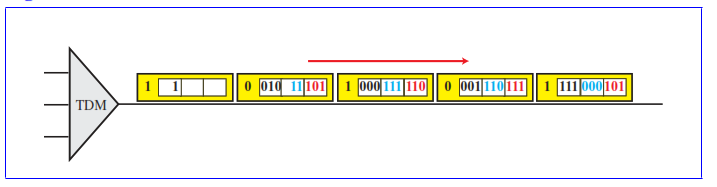
\includegraphics[width=0.9\textwidth]{solusi12.png}
\end{figure}

\vspace{12pt}

\begin{exercise}
  Contoh soal 13 : Gambar 3.1 dibawah menunjukkan demultiplexer dalam TDM sinkron. Jika slot input adalah 16 bit
  panjang (tanpa bit framing), apa aliran bit di setiap output? Bit tiba di
  demultiplexer seperti yang ditunjukkan oleh panah.

  \begin{figure}[h]
    \centering
    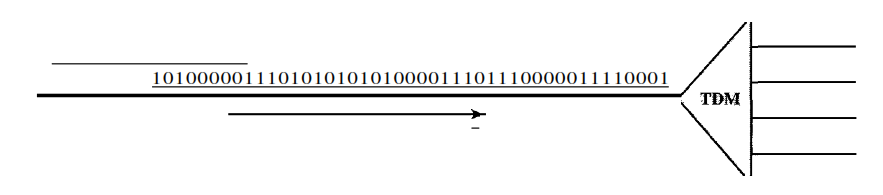
\includegraphics[width=0.9\textwidth]{soal13.png}
    \caption{TDM}
  \end{figure}

\end{exercise}


\vspace{40pt}

\begin{solution}
  \begin{figure}[h]
    \centering
    
\includegraphics[width=0.9\textwidth]{solusi13.png}
    \caption{solusi TDM}
  \end{figure}
\end{solution}




\begin{exercise}
  Jawab pertanyaan berikut tentang hierarki digital pada Gambar 3.3:
  \begin{itemize}
    \item[a.] Berapa overhead (jumlah bit tambahan) dalam layanan DS-l?
    \item[b.] Berapa overhead (jumlah bit tambahan) dalam layanan DS-2?
    \item[c.] Berapa overhead (jumlah bit tambahan) dalam layanan DS-3?
    \item[d.] Berapa overhead (jumlah bit tambahan) dalam layanan DS-4?
  \end{itemize}
\end{exercise}

\begin{figure}[h]
  \centering
  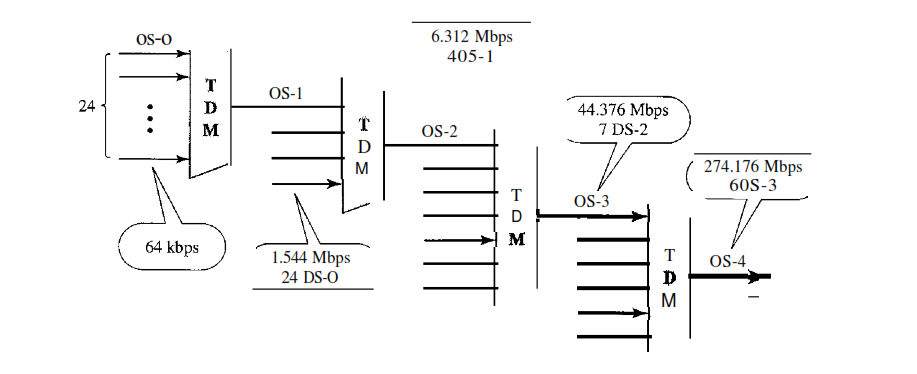
\includegraphics[width=0.9\textwidth]{figure6.23.png}
  \caption{Hierarki Digital}
\end{figure}

\begin{solution}
  \begin{itemize}
    \item[a.] DS-1 Overhead = 
    \begin{math}
       1.544 Mbps - (24 \times 64 kbps) = 8 kbps 
    \end{math}
   \item [b.] DS-2 Overhead =
        \begin{math}
          6.312 Mbps - (4 \times 1.544 kbps) = 136 kbps 
        \end{math}
   \item [c.] DS-3 Overhead =
        \begin{math}
          44.376 Mbps - (7 \times 6.312 kbps) = 192 kbps 
        \end{math}
   \item [d.] DS-4 Overhead =
   \begin{math}
    274.176 Mbps - (6 \times 44.376 kbps) = 7.92 Mbps 
  \end{math}
  \end{itemize}
\end{solution}

\vspace{12pt}

% Maranti Nainggolan 15-18
\begin{exercise}
  Contoh soal 15
\end{exercise}

\begin{solution}
  Contoh solusi
\end{solution}

\vspace{12pt}

\begin{exercise}
  Contoh soal 16
\end{exercise}

\begin{solution}
  Contoh solusi
\end{solution}

\vspace{12pt}

\begin{exercise}
  Contoh soal 17
\end{exercise}

\begin{solution}
  Contoh solusi
\end{solution}

\vspace{12pt}

\begin{exercise}
  Contoh soal
\end{exercise}

\begin{solution}
  Contoh solusi
\end{solution}

\end{document}

